\documentclass{article}

\usepackage[a4paper]{geometry}
\usepackage{graphicx}
\usepackage[utf8]{inputenc}
\usepackage{subcaption}
\usepackage{placeins}
\usepackage{wrapfig}
\usepackage{float}
\usepackage{minted}
\usepackage[noEnd=false, indLines=false]{algpseudocodex}
\usepackage{hyperref}
\usepackage{tikzit}
\input{Tema1styles.tikzstyles}

\graphicspath{{./images/}}

\newcommand{\code}[2]{\inputminted[linenos, breaklines, firstline=#1, lastline=#2]{c++}{Tema1.cpp}}

\title{Tema 1 --- Sortarea topologică}
\author{
    Mițca Dumitru\\
    Grupa NNNNL
}
\date{2023}

\begin{document}
    \maketitle

    \hypersetup{linkbordercolor=1 1 1}
    \renewcommand*\contentsname{Cuprins}
    \tableofcontents
    \hypersetup{linkbordercolor=1 0 0}

    \newpage

    \section{Prezentarea problemei}

    Problema sortării este o problemă foarte populară în informatică, pentru care zeci de algoritmi
    au fost propuși, algoritmi fie inovativi (quicksort, merge sort), sau care rafinează algoritmi
    existenți (timsort\footnote{Folosit de Python, derivat din merge sort și insertion sort:
    \url{https://bugs.python.org/file4451/timsort.txt}}, glidesort\footnote{Derivat din quick sort
    și merge sort: \url{https://github.com/orlp/glidesort}}).

    Sortarea topologică în particular poate fi folosită în planificarea unei serii de job-uri sau
    task-uri, deoarece există posibilitatea modelării acestora și dependențelor lor folosing grafuri.
    Câteva exemple de aplicații ale sortării topologice sunt planificarea execuției instrucțiunilor,
    alegerea ordinii executării task-urilor într-un Makefile sau rezolvarea dependențelor între
    simbolori de către link-editor.

    \section{Prezentarea algoritmului}

    Algoritmul este următorul:

    \begin{algorithmic}
        \Procedure{sortareTopologicaBFS}{D, np}
            \State coadaVida(C)
            \For{$u \gets 0 $ \textbf{to} $ D.n-1$}
                \If{$D.np[u] = 0$} \Comment A
                    \State insereaza(C, u)
                \EndIf
            \EndFor
            \For{$k \gets 0$ \textbf{to} $D.n-1$}
                \If{esteVida(C)} \Comment B
                    \State \Return ("Graful conține cicluri")
                \EndIf
                \State $u \gets$ elimina(C)
                \State insereaza(L, u)
                \State $p \gets D.a[u]$
                \While{$p \neq \texttt{NULL}$}
                    \State $v \gets p$\texttt{->}$elt$
                    \State $D.np[v] \gets D.np[v] - 1$
                    \If{$D.np[v] = 0$}
                        \State insereazaa(C, v)
                    \EndIf
                \EndWhile
            \EndFor
        \EndProcedure
    \end{algorithmic}

    Algoritmul plasează noduri înaintea succesorilor lor, astfel asigurându-se că relație de ordine
    definită de graf este respectată.

    \texttt{if}-ul marcat cu \textbf{B} va fi atins în următoarele situații:
    \begin{itemize}
        \item un ciclu nu este atașat niciunui drum care conține noduri ce nu participă în cicluri,
        astfel niciun nod din ciclu nu va intra în coada \emph{C} deoarece \texttt{if}-ul marcat cu
        \textbf{A} previne acest lucru
        \item un ciclu atașat unui drum care conține noduri care nu participă in cicluri, deoarece
        numărul de predecesori pentru măcar un nod nu va deveni 0, ceea nu va permite adăugarea
        nodului în coada \emph{C}, nepermițând astfel explorarea succesorilor acelui nod
    \end{itemize}

    Ambele cazuri duc la situația în care coada este goală, dar totuși au rămas noduri de explorat
    (ceea ce înseamnă că codul nu va ieși din \texttt{for}-ul normal, ci abrupt prin \texttt{return}-ul
    aferent \texttt{if}-ului \textbf{B}).

    \section{Prezentarea programului}

    Programul începe incluzând librăriile necesare lui:
    \code{1}{5}

    Apoi urmează declararea structurii care va reprezenta digraful în cod:
    \code{7}{21}

    Și definirea tipului de excepție care va fi folosit de algoritm pentru a semnala erori:
    \code{23}{28}

    După acestea, urmează o traducerea foarte loială a pseudocodului algoritmului oferit în cerință,
    excepție făcând lucrul cu liste simplu înlănțuite, care a fost realizat folosind \texttt{std::list}
    din biblioteca standard, în locul implementării manuale presupuse de algoritm:
    \code{30}{66}

    Și intr-un final funcția \texttt{main}, care pur și simplu rulează algoritmul, verificând dacă
    apar erori și care afișează nodurile în ordine topologică, în caz contrar:
    \code{68}{96}

    \section{Rulări}

    Pentru graful:
    \ctikzfig{Tema1nocycles}
    Rezultatul este:
    \begin{figure}[H]
        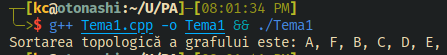
\includegraphics[width=0.75\linewidth]{Tema1Rulare1}
        \centering
        \caption{Rezultatul rulrii pe un graf care nu conține cicluri}
    \end{figure}


    Iar pentru graful:
    \ctikzfig{Tema1cycles}
    Rezultatul este:
    \begin{figure}[H]
        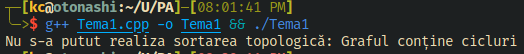
\includegraphics[width=0.75\linewidth]{Tema1Rulare2}
        \centering
        \caption{Rezultatul rulării pe un graf care conține cicluri}
    \end{figure}

    Pentru graful:
    \ctikzfig{Tema1anothercycle}
    Rezultatul este:
    \begin{figure}[H]
        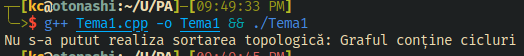
\includegraphics[width=0.75\linewidth]{Tema1Rulare3}
        \centering
        \caption{Rezultatul rulării pe un graf care conține cicluri plasate pe un drum}
    \end{figure}
\end{document}
